\subsection{Task 2: Pagerank}
In this experiment, we run pagerank on various size of graph data, 10 in total. The purpose of this design is that we think pagerank is a time consuming operation, and our first try proves our intuition. So we want to test the implementation on incrementally larger dataset, so that we can spot the bottleneck of single machine implementation. 

\begin{center}
\begin{tabular}{| c | c | c |}
    \hline
    Roadnet-ca & 1,965,206 & 5,533,214 \\ \hline
    Roadnet-PA & 1,088,092 & 3,083,796 \\ \hline
    Roadnet-TX & 1,379,917 & 3,843,320 \\ \hline
    com-Amazon & 334,863 & 925,872 \\ \hline
    web-BerkStan & 685,230 & 7,600,595 \\ \hline
    email-Enron & 36,692 & 367,662 \\ \hline
    web-Google & 875,713 & 5,105,039 \\ \hline
    soc-Slashdot0902 & 77,360 & 905,468 \\ \hline
    web-Stanford & 281,903 & 2,312,497 \\ \hline
    wiki-Vote & 7,115 & 103,689 \\ \hline
\end{tabular}
\end{center}

\subsubsection{Plot}
Please refer to Figure \ref{t2:1}.

\begin{figure}[!h]
\begin{center}
\begin{tabular}{c c c}
     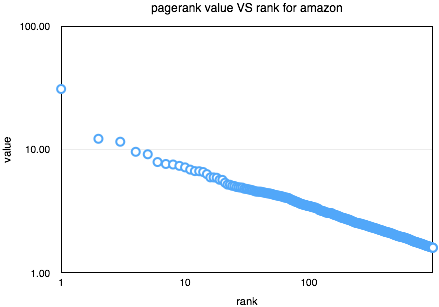
\includegraphics[width=0.3\textwidth]{FIG/t2_amazon.png} &
     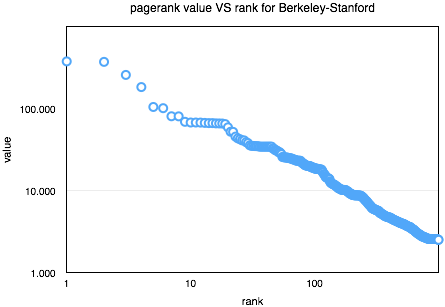
\includegraphics[width=0.3\textwidth]{FIG/t2_berke.png} &
     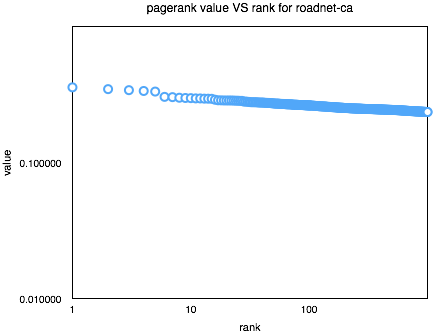
\includegraphics[width=0.3\textwidth]{FIG/t2_ca.png}\\
    (a) & (b) & (c)\\
     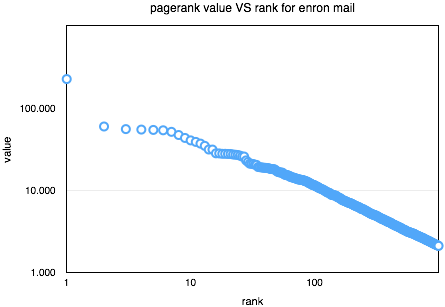
\includegraphics[width=0.3\textwidth]{FIG/t2_enron.png} &
     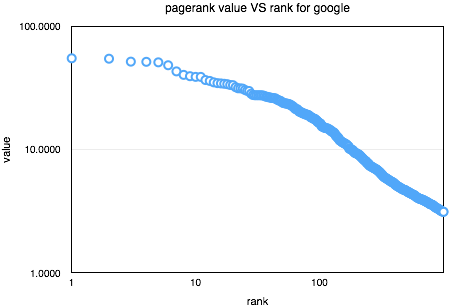
\includegraphics[width=0.3\textwidth]{FIG/t2_google.png} &
     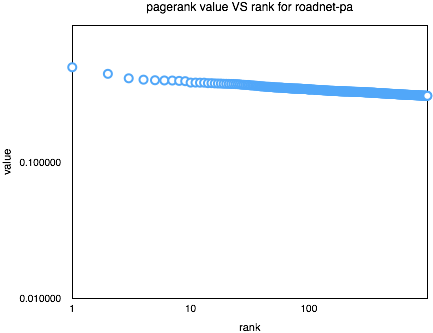
\includegraphics[width=0.3\textwidth]{FIG/t2_pa.png} \\
     (d) & (e) & (f)\\
     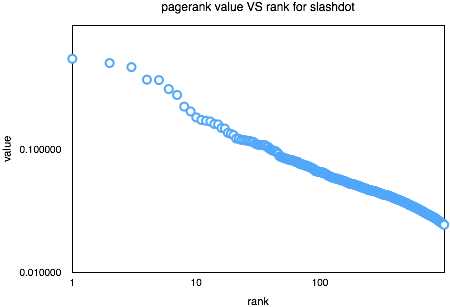
\includegraphics[width=0.3\textwidth]{FIG/t2_slashdot.png} &
     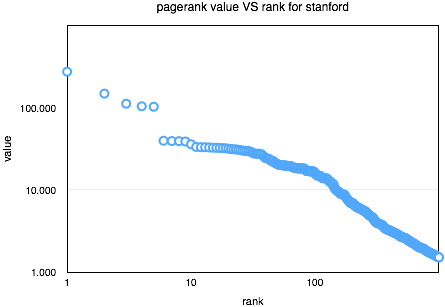
\includegraphics[width=0.3\textwidth]{FIG/t2_stanford.png} &
     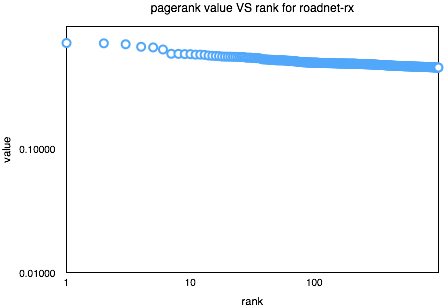
\includegraphics[width=0.3\textwidth]{FIG/t2_tx.png}\\
     (g) & (h) & (i)\\
     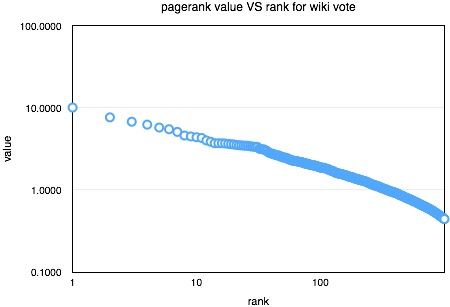
\includegraphics[width=0.3\textwidth]{FIG/t2_wikivote.png} & &\\
     (j) & &
\end{tabular}
\caption{Rank-frequency plot for Task 2. (a)Amazon (b)Berkeley-Stanford web graph (c)Roadnet-CA (d)Enron Mail (e)Google web graph (f)Roadnet-PA (g)Slashdot (h)Stanford (i)Roadnet-TX (j)Wiki vote}
\label{t2:1}
\end{center}
\end{figure}

\subsubsection{Observation}
We can observe that in log-log scale, all datasets exhibits linear relationship between rank and frequency. Thus we find another appearance of power law in natural graph. An abnormal phenomenon is that the slope of Roadnet datasets is nearly flat. This reflects another aspects of the fundamental property of Roadnet, that all nodes in a roadnet graph are nearly equal to each other, it's a decentralized graph. While in ordinary social network, we always expect to have some important authorities. 




